\documentclass[11pt,a4paper]{article}
\usepackage[utf8]{inputenc}
\usepackage{amsmath}
\usepackage{pdflscape}
\usepackage{hyperref}
\usepackage{amsfonts}
\usepackage{float}
\usepackage{graphicx}
\usepackage{amssymb}
\usepackage{parskip}
\title{\vspace{-2.0cm} \textbf{SENG 300: Assignment 3}}
\author{Celina Ma, John Ngo, Omar Qureshi}
\begin{document}
\maketitle
\def\textfraction{.01}
\def\topfraction{.99}
\section*{Deliverable \#1}

\subsection*{1-1: Poker Effort Estimation}

For our planning poker session, we chose to create tasks for the following functional requirement:

\textbf{The app must process event data from the muon detector to determine the number of events per minute over a specific time interval.}

We generated six tasks for this functional requirement and individually rated the difficulty of each task from one to ten. During our planning session, we generally had consensus for our ratings, with some variance between us. 

For example, the task, “Create an addEvent method to store processed MuonEvents to an array”, was considered to be relatively easy by all of us. However, one person rated the difficulty slightly higher and suggested that this method may need to check if the event data is valid (eg. if the timestamps are in an order that makes sense). We discussed some other issues that may occur, such as what should happen if a maximum number of events had been reached. These additional factors helped clarify the difficulty of the task.

The task of “calculating the difference in minutes between two timestamps” was more divisive. One of our group members believed the task would be quite difficult (7) but another believed it would be easy (3), since Java likely contained some built-in functionality to help with the task. We learned that this was indeed the case and adjusted our rankings accordingly.
We all agreed that the task of “calculating events per minute over a specific time interval” would be difficult. During our discussion, we contemplated how the number of events per minute could be displayed “live” on our app screen while collecting data, since that would involve frequently saving new timestamps for the calculation. We also wondered if events per minute should only be calculated over some fixed time interval (eg. the last 10 seconds of recording) or use the whole time spent recording.

Overall, the planning poker session was useful for evaluating our list of tasks by raising new questions on generating ideas for test cases and structure.


\subsection*{1-2: Silent Grouping Effort Estimation}

Once our planning poker session was completed, we moved along to do silent grouping effort estimation. We now had to define features of the functional requirement rather than the tasks. The definition of a feature we used was an element the user can see or interact with, corresponding to the functional requirement defined in \textit{Deliverable 1-1}. The features we came up with were:

\begin{enumerate}

\item The user is able to press the 'Start Recording' button to begin when data collection starts.
\item The user is able to see events being displayed on the recording screen after each new event is detected and added.
\item The user is able to stop the recording midway if desired.
\item The user is able to clear the screen once a session is done to start a new recording session.
\item The user is able to see when a recording is in progress by noticing the green Start Recording button changes into a red Recording (duration remaining in s) button.
\end{enumerate}

After coming up with the above list, we wrote them down on some post-it notes and used a table rather than a wall to do the sorting;

\begin{figure}[h]
\centering
	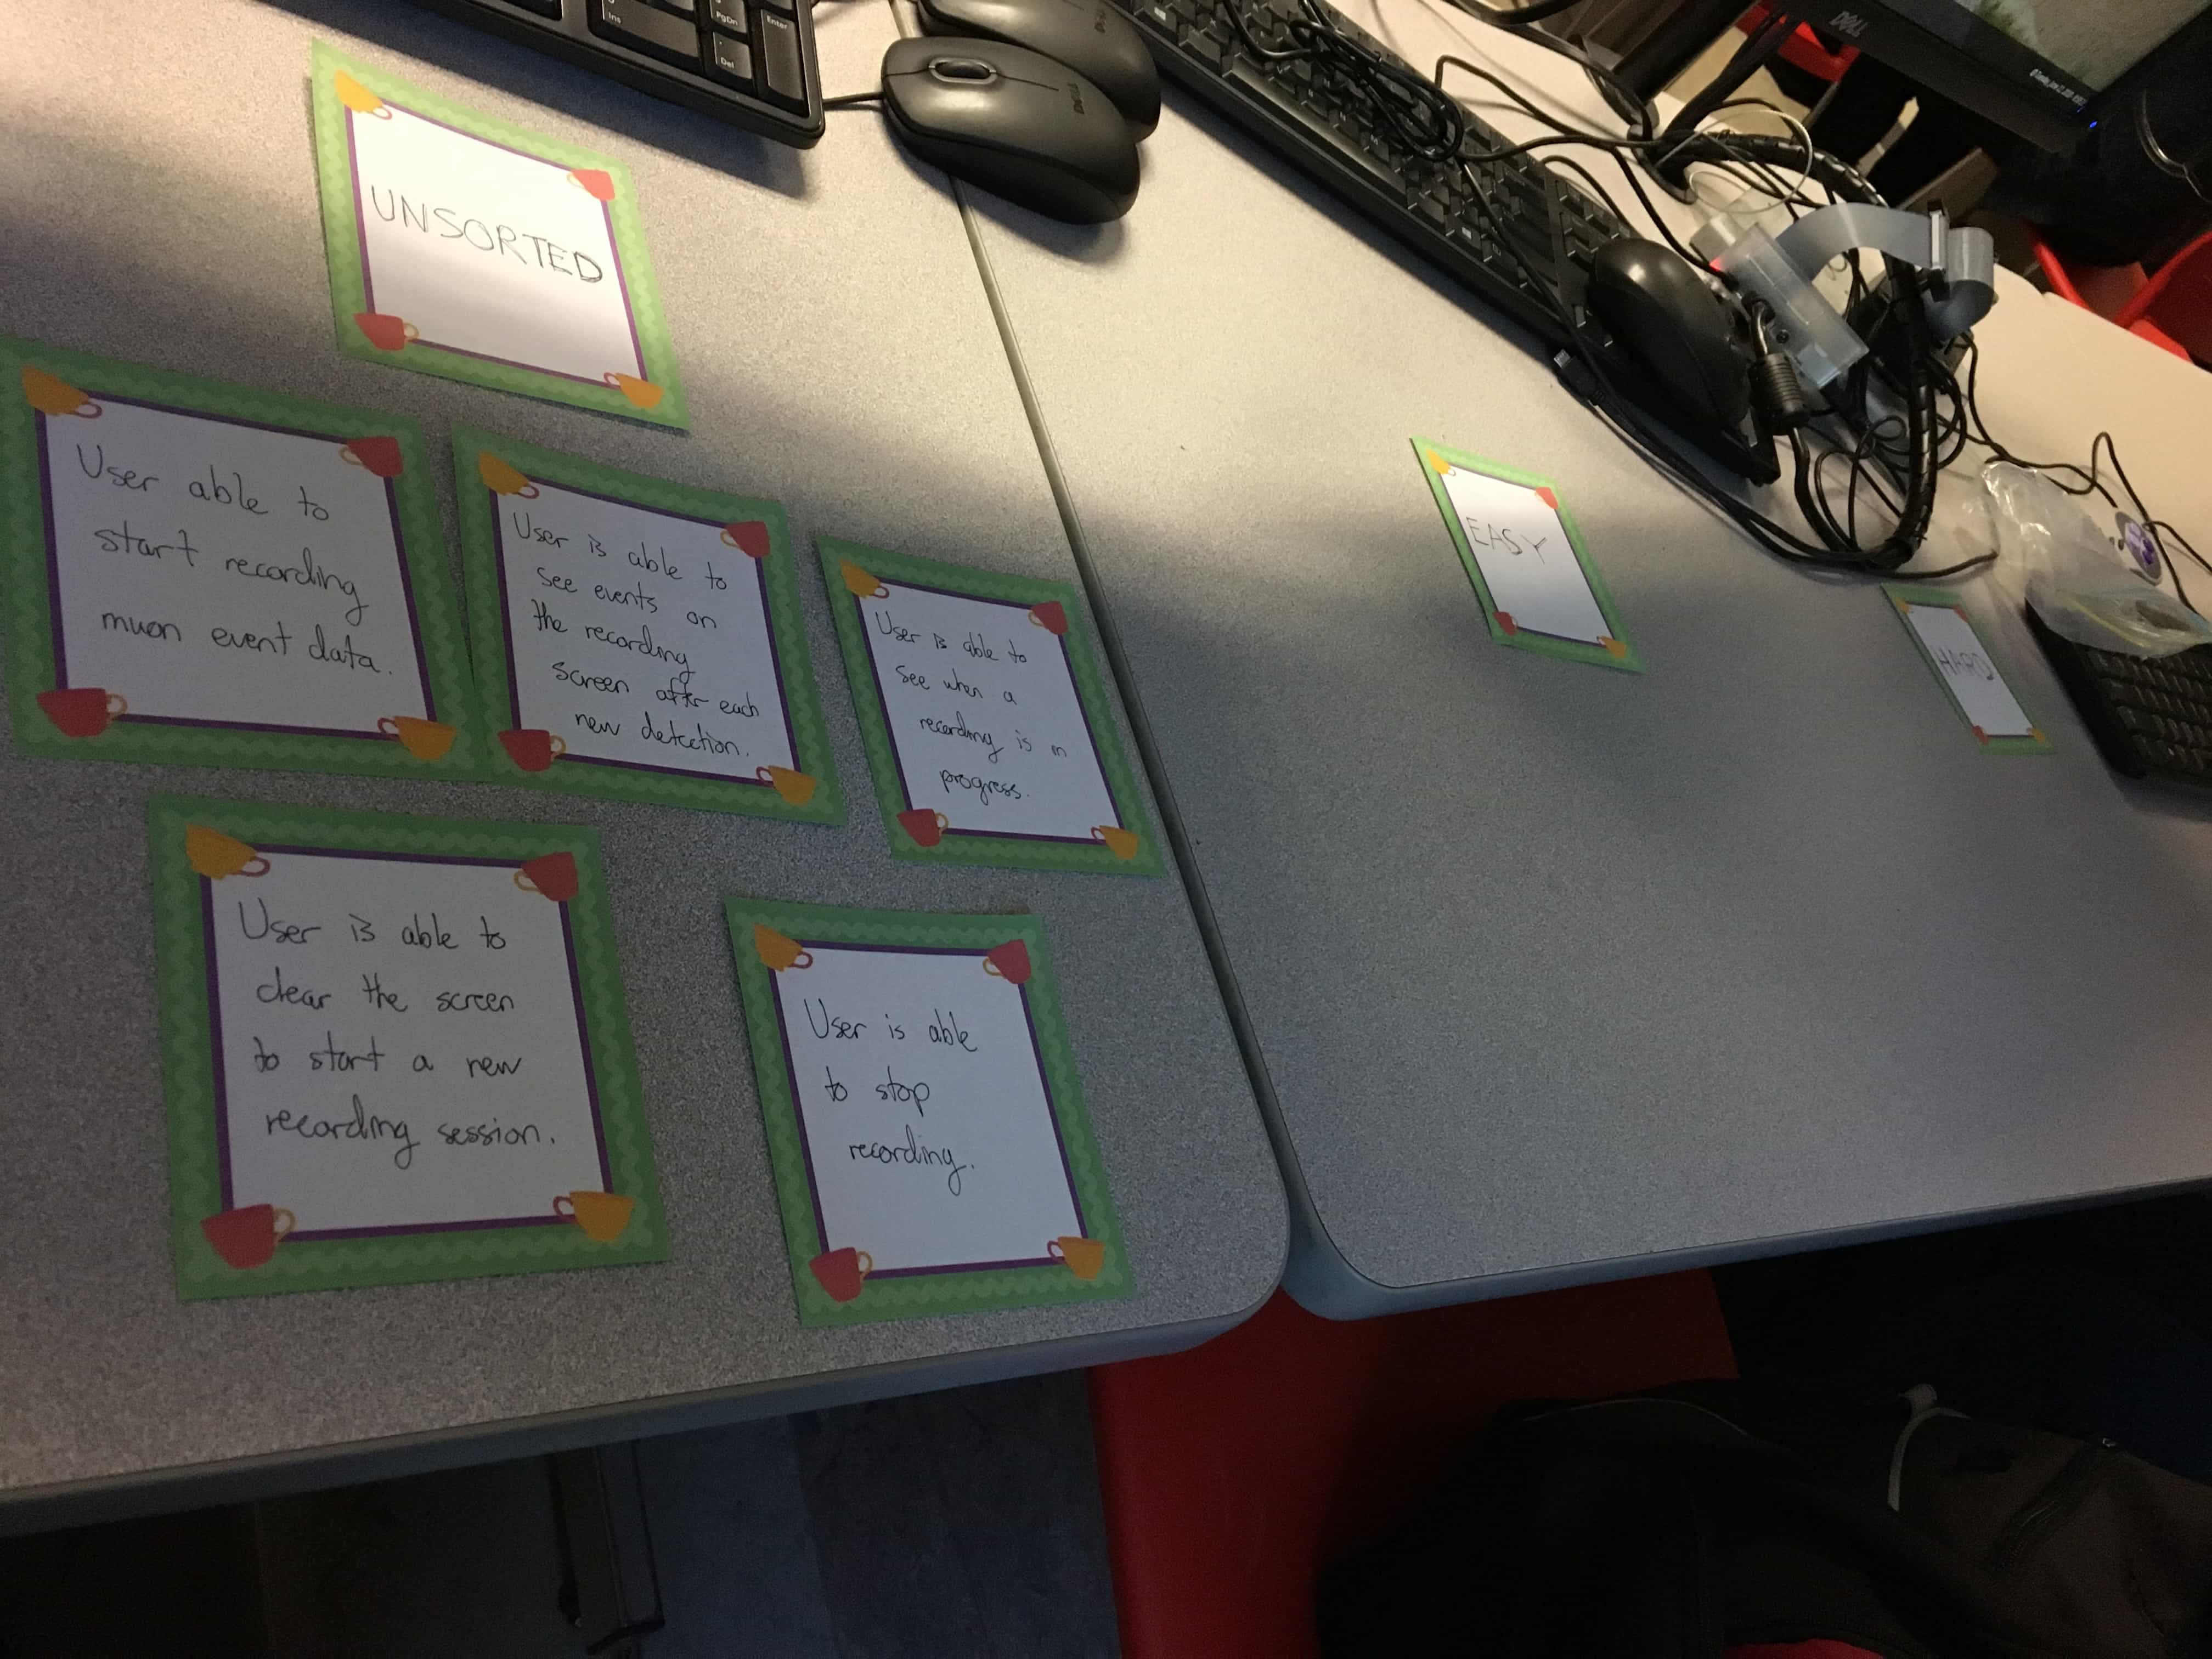
\includegraphics[width=0.9\textwidth]{silentimg1.png}
	\caption{Post it notes started initially in the unsorted pile and a table was used for convenience}
\end{figure}

\newpage

One of the issues we noticed with the silent grouping method was the lack of granularity of the piles. A feature was either easy or hard whereas the planning poker method was able to give a finer sense of difficulty. As such, clearly easy or hard features were the first to get picked and sorted which is seen in the below in progress shot; 

\begin{figure}[h]
	\centering
	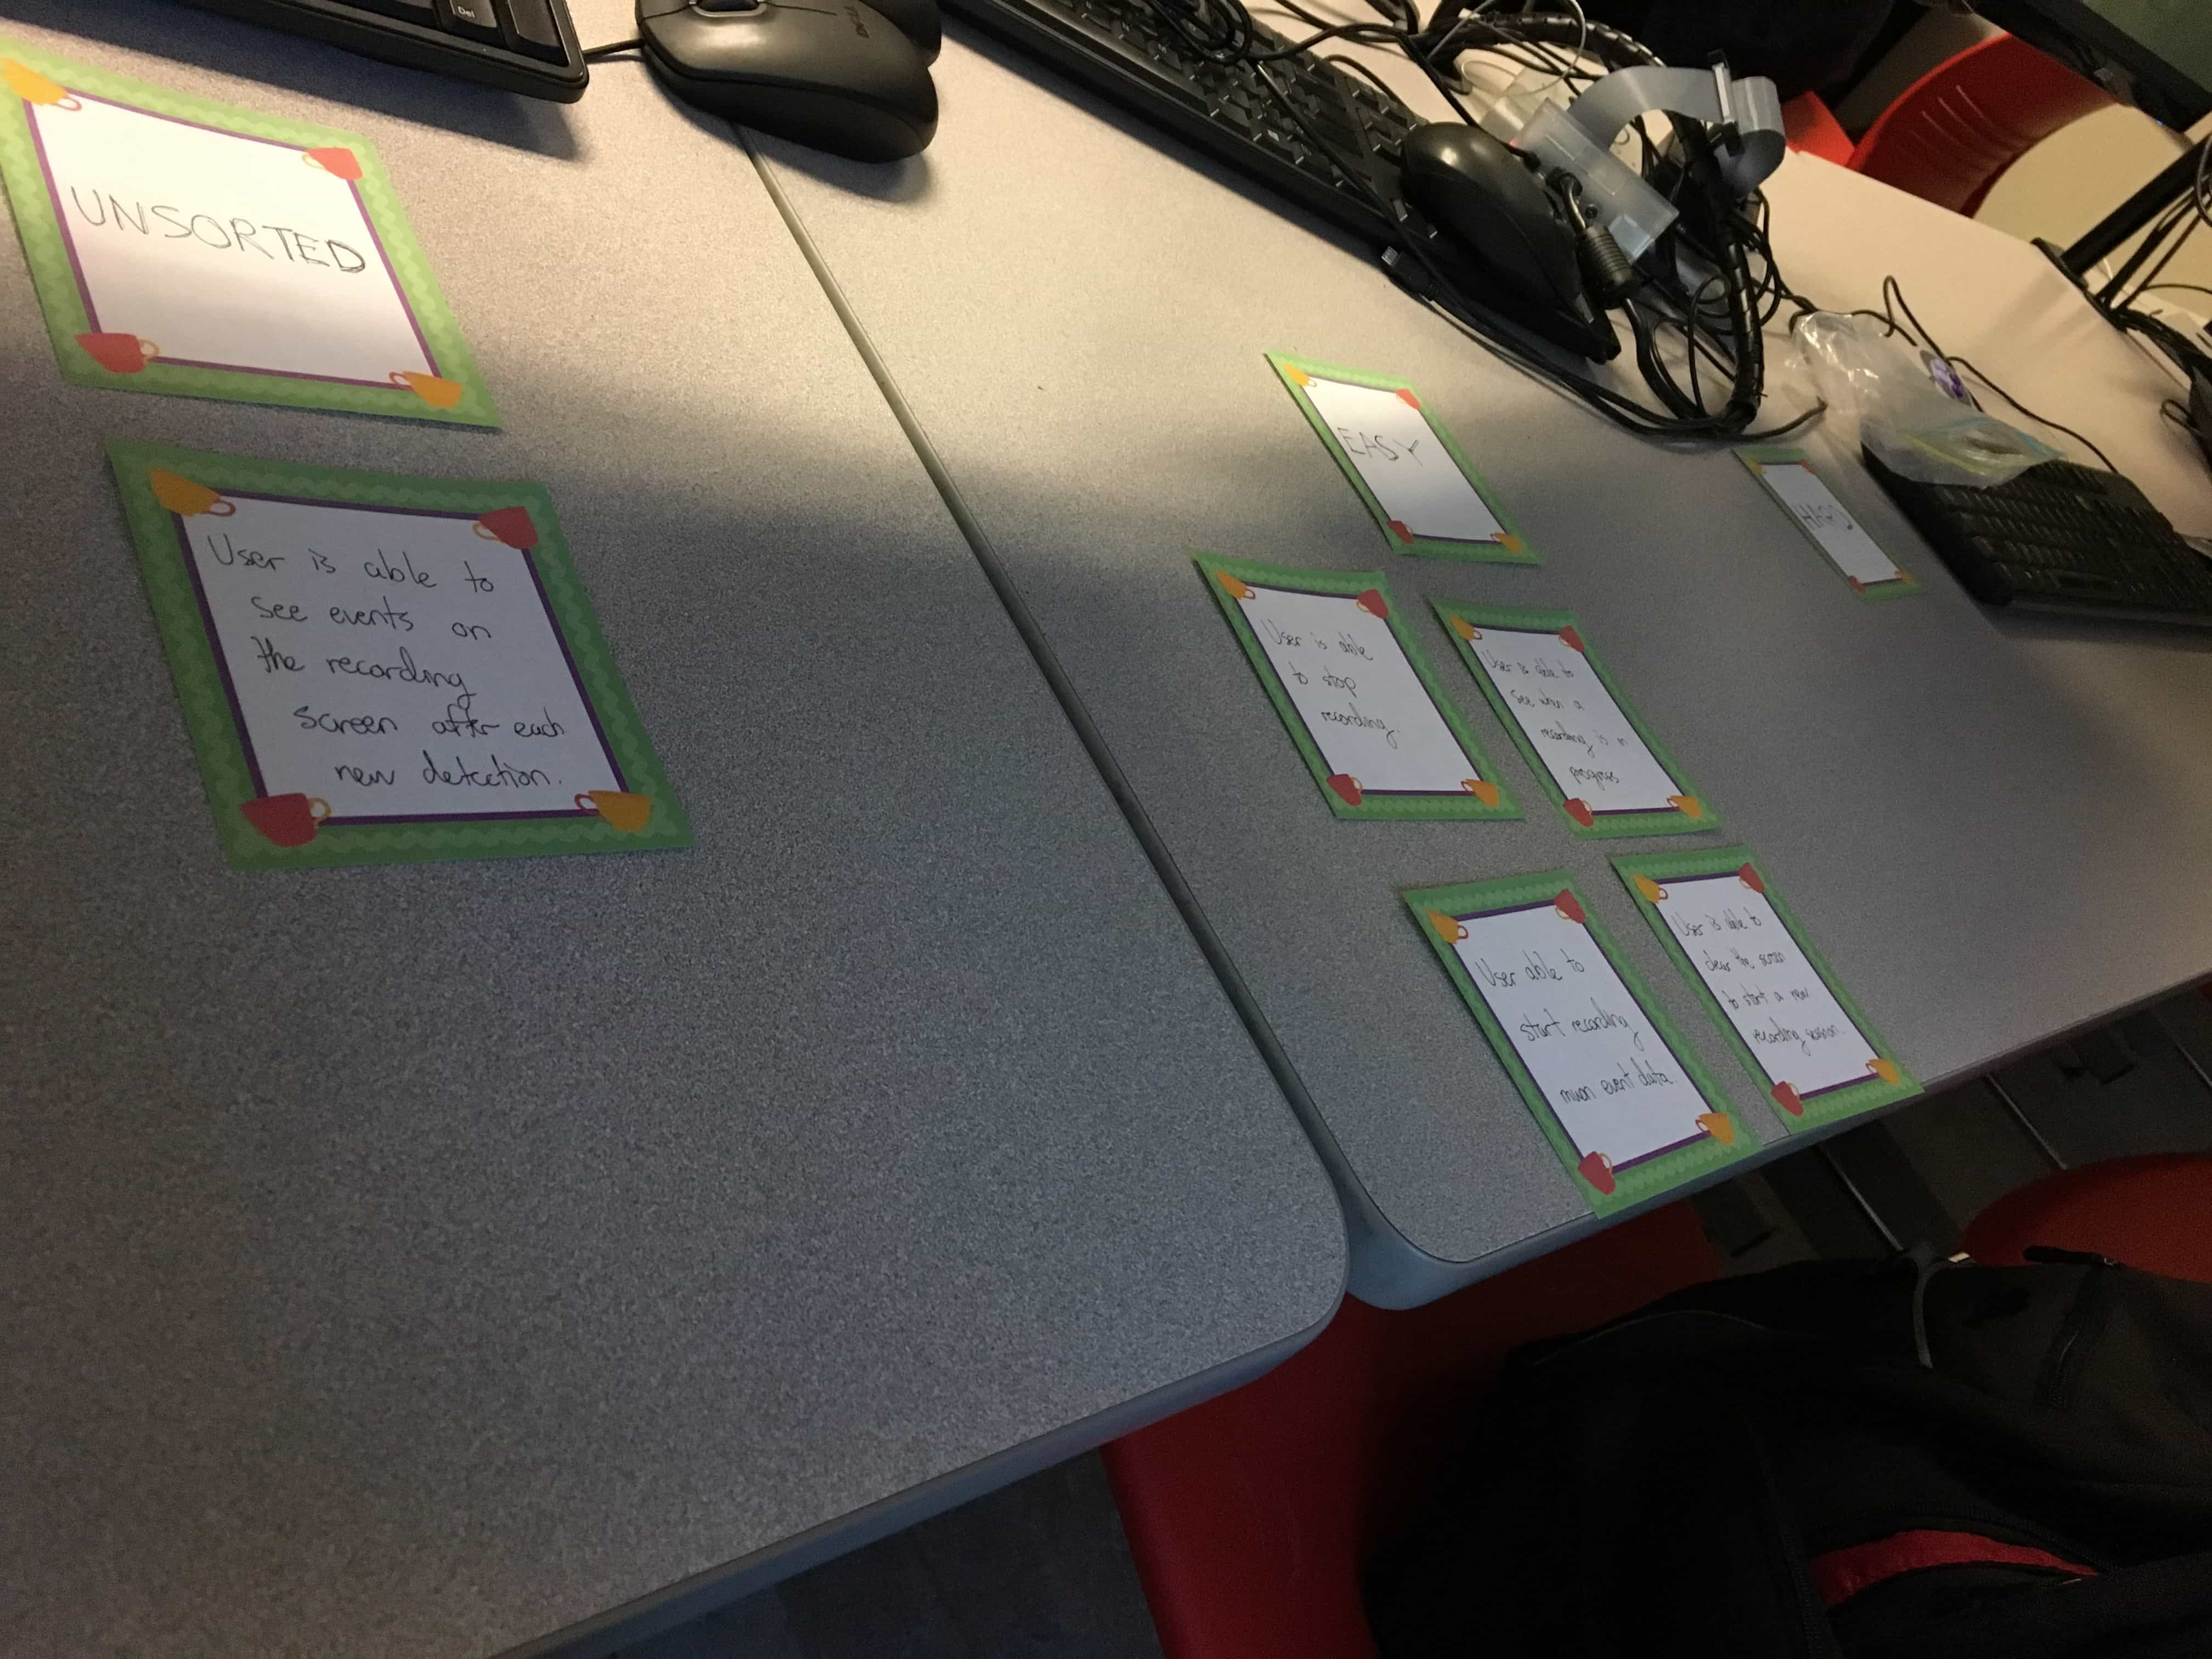
\includegraphics[width=0.5\textwidth]{silentimg2.png}
	\caption{Silent grouping effort estimation in progress}
	\end{figure}

We then attempted to categorize some of the harder features such as displaying the live event being detected and added to a running total. This aligned with our previously defined hard task in \textit{Deliverable 1-1} and a consensus was reached that this would indeed be difficult. 

Afterwards, a feature that was hard to reach an agreement on was stopping the recording half way. Stopping it mid way may prove to be difficult so after a few back and forth for that feature, we decided to put it in a middle 'hold' section as seen below:

\begin{figure}[h]
	\centering
	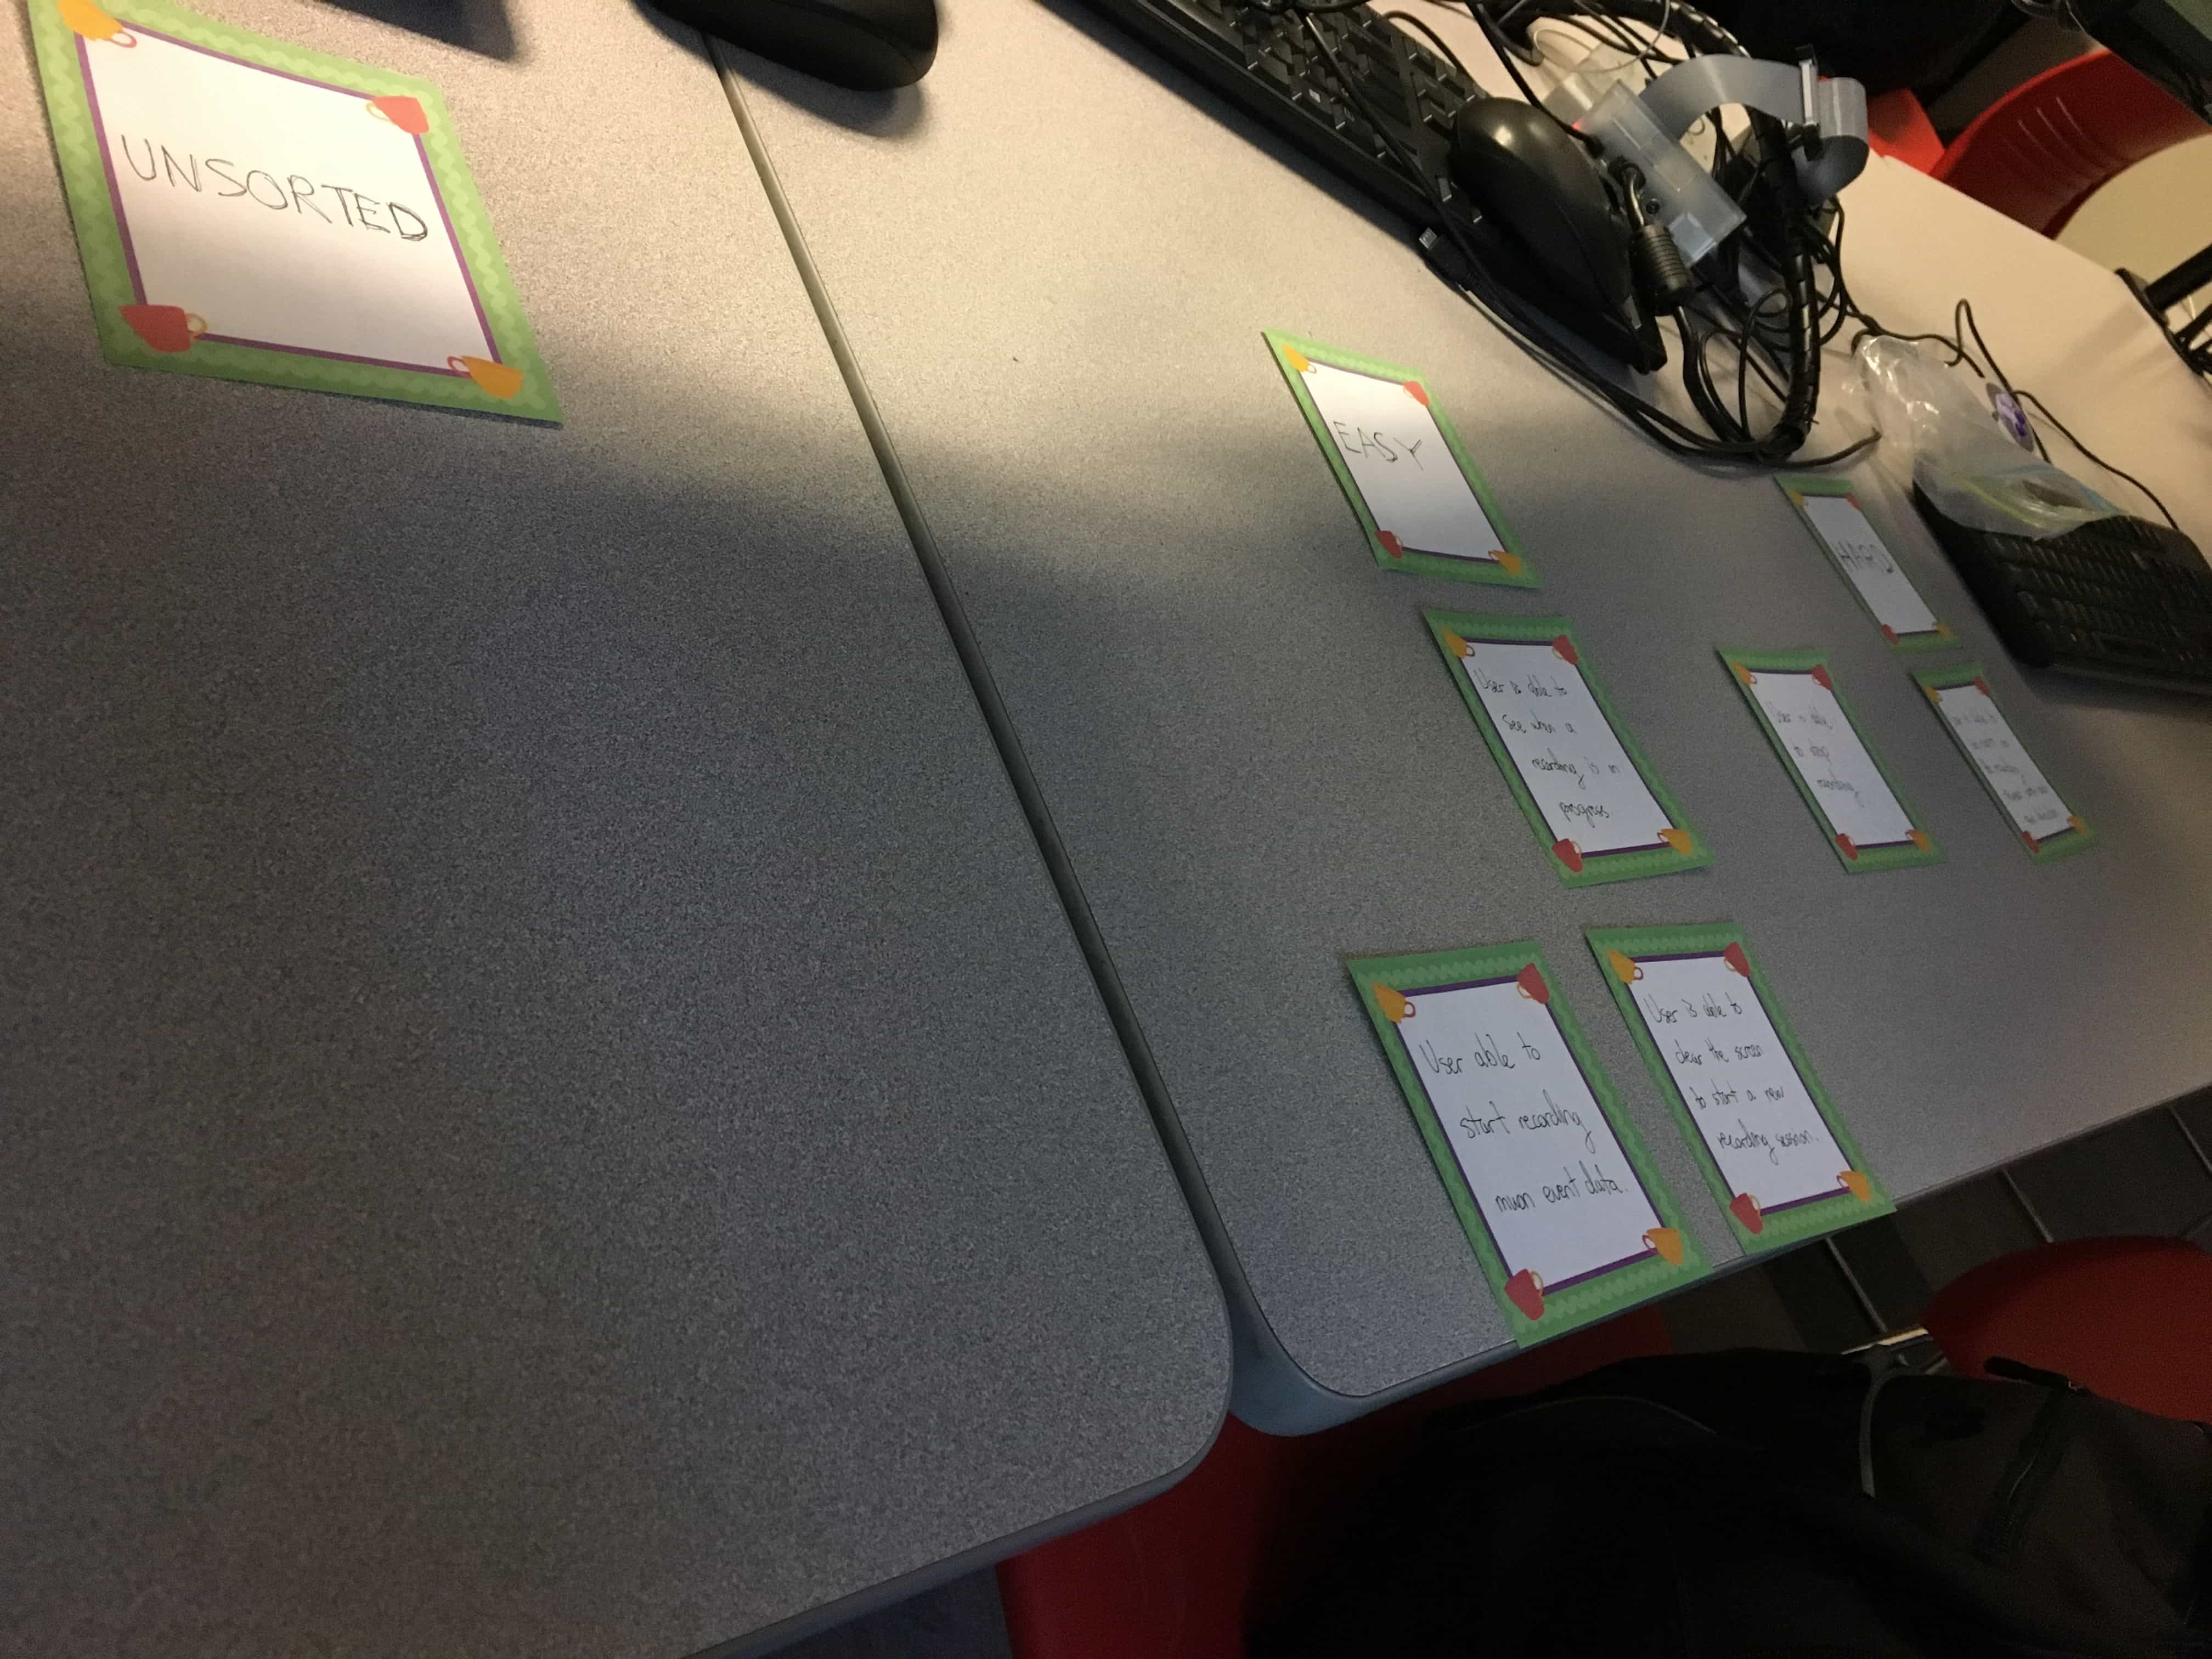
\includegraphics[width=0.5\textwidth]{silentimg3.png}
	\caption{Completed session with one of the features being placed on hold}
	\end{figure}
	
Overall, silent grouping  proved to be a valuable medium of communication in allowing team members to interact with one another. An exchange of different views can ultimately help in creating a better application. 


\newpage
\section*{Deliverable \#2}

\subsection*{2-1: Task Breakdown}

\begin{figure}[h]
  \centering
      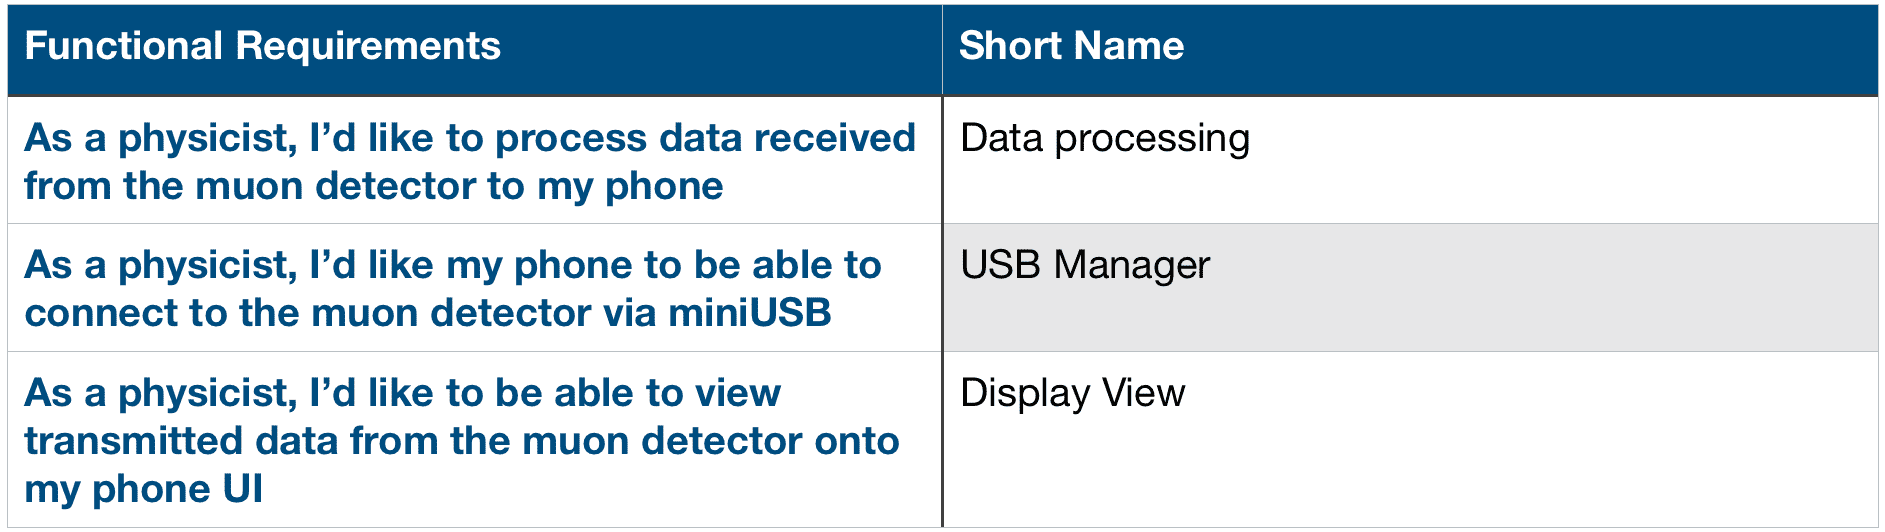
\includegraphics[width=1\textwidth]{table1.png}  
\end{figure}

Our first table shows the three main functional requirements picked for the app and their corresponding short names to be used in the following tables.

\begin{figure}[h]
  \centering
      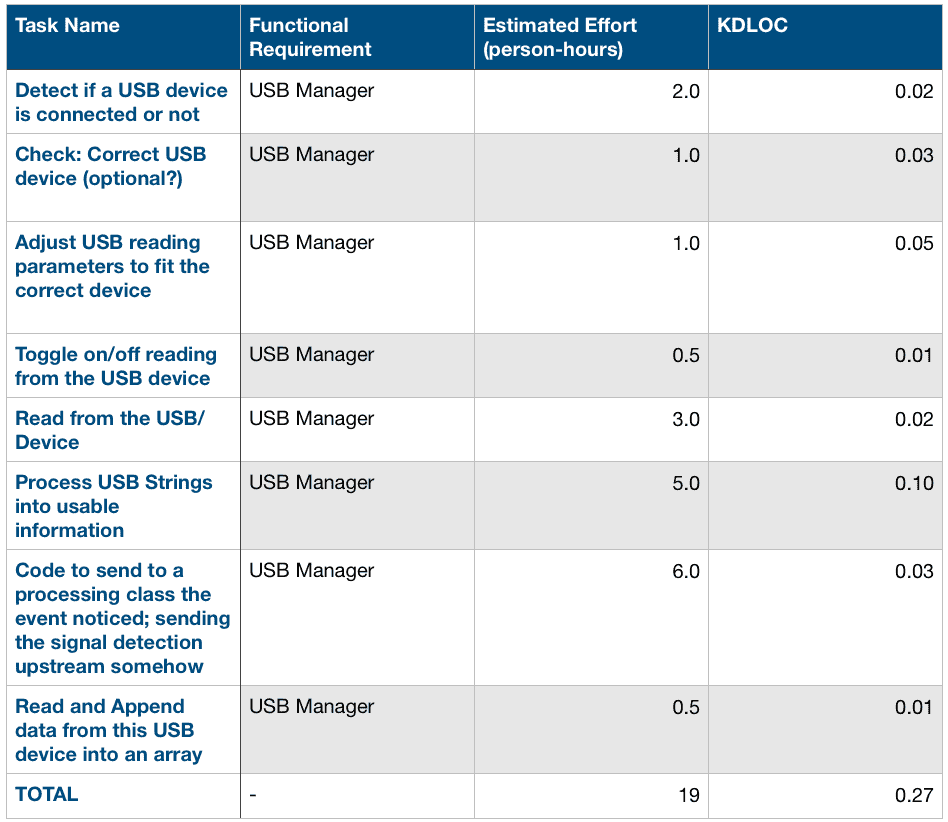
\includegraphics[width=1.0\textwidth]{USBMtable3.png}  
\end{figure}

Our second table corresponds to the USB Manager functional requirement. The table format serves as a visual aid for breaking down requirements into tasks and effort, which also provides a documentation reference in the future for cost estimation. 

\newpage
\begin{figure}[h]
  \centering
      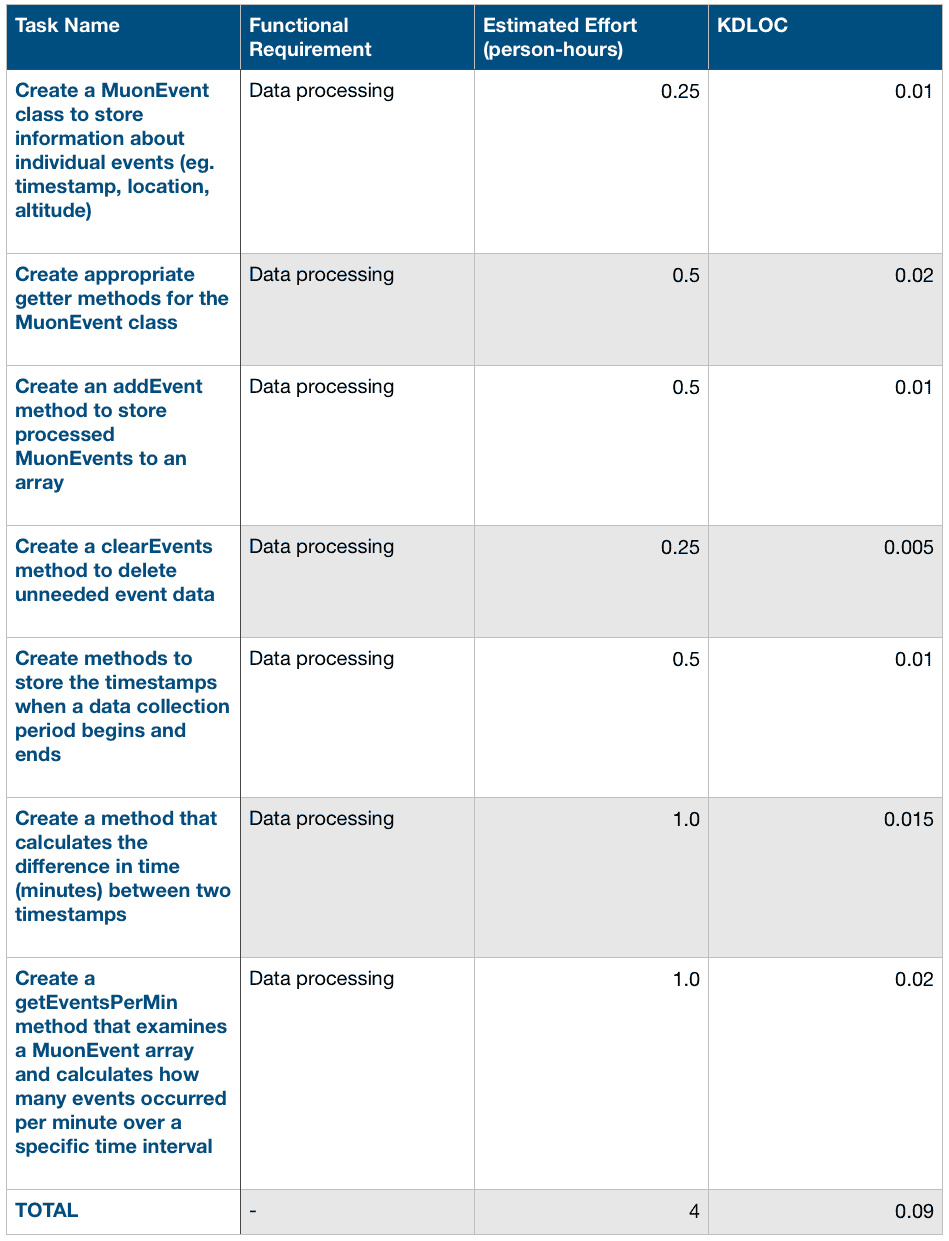
\includegraphics[width=1.0\textwidth]{dataproctable2.png}  
\end{figure}

Our second requirement is similarly broken down into individual tasks and their corresponding estimated effort.

\newpage
\begin{figure}[h]
  \centering
      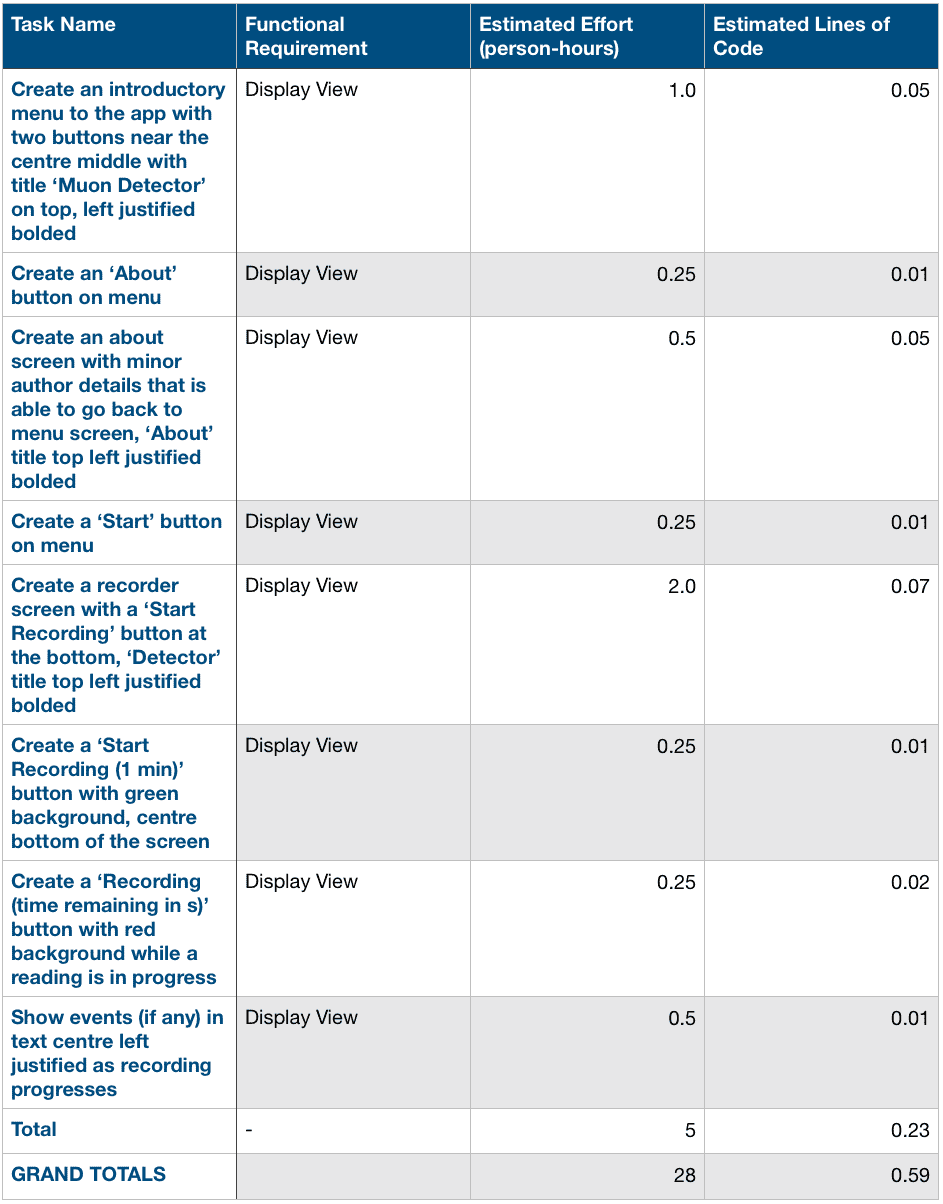
\includegraphics[width=1.0\textwidth]{displaytable4.png}  
\end{figure}

Finally, our third table for the final display functional requirement is also broken down. 

Overall, this exercise in the design process helped create estimates on the challenges to be faced when completing functionality of the application. This also helped plan our schedules since we now had a general idea of time required for each step. 

\newpage
\subsection*{2-2: Effort Estimation using Intermediate COCOMO Model}

\textbf{Project type:} Semi-Detached (a = 3.0, b = 1.12)

\textbf{Justification:} Our project can best be described as a semi-detached project. While part of our project involves data processing and data retrieval, the other half is hardware based in that it depends on communication through USB with a scientific instrument. The overall project is ambitious for our team, since we have fairly little experience with much of the components of the project, incl. Android programming and USB interaction. The app is being developed by a small team, and ultimately aims to have real-time display of detection events as fed through by the USB link. As such, straddling the lines of organic and embedded as it is, it stands to reason that the project is semi-detached.

The following table represents our Cocomo factors along with their associated cost ratings, which will be used in the equation to calculate our person-hours:

\begin{figure}[h]
\centering
      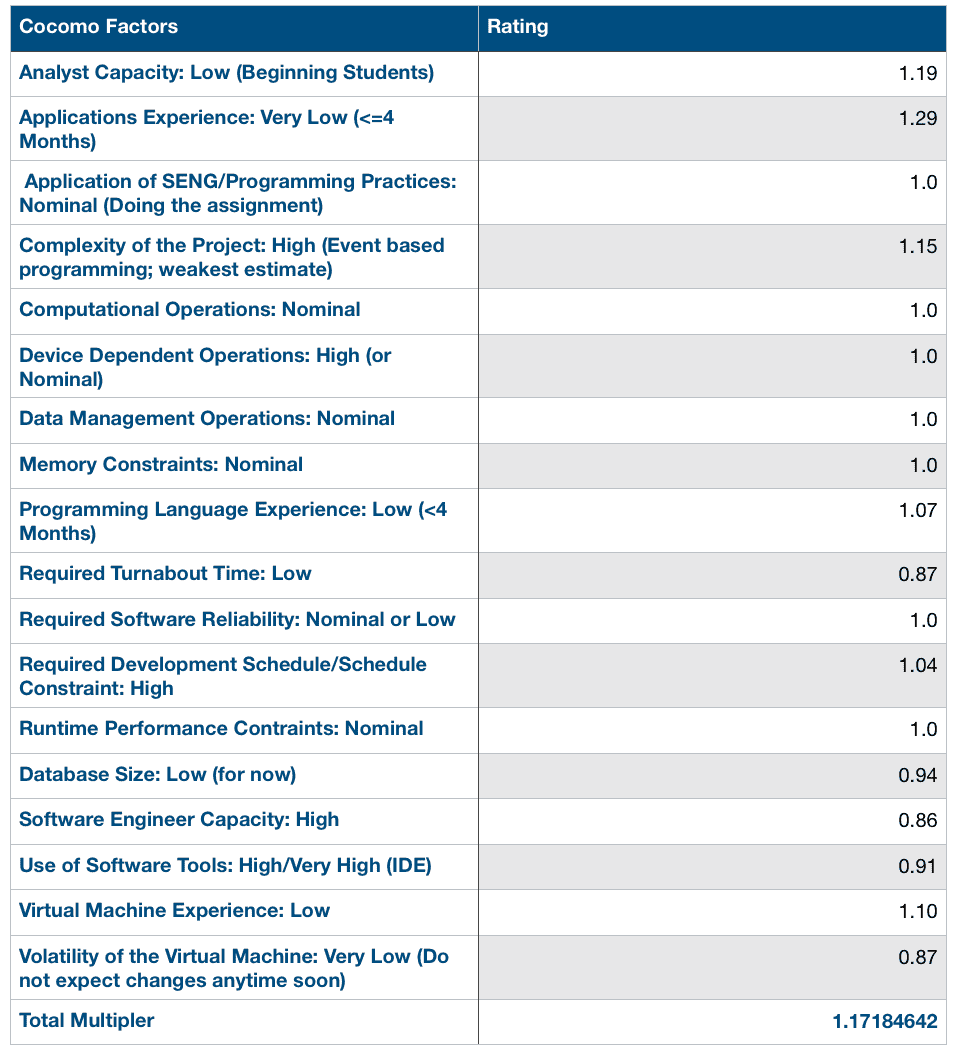
\includegraphics[width=0.85\textwidth]{cocoimg1.png}  
\end{figure}

Of the cost driver factors, this is the justifications for why some of the factors may be different from nominal:

\begin{enumerate}
\item Analyst Capacity: Our analyst capacity is low, because we are software engineering students in our first software engineering class, just beginning to apply what we've learned here. As such, we have little confidance in our own analysis capacities.
\item Applications Experience: We selected very low here because none of us have worked on a comparable project before. We haven't worked on android before, we haven't worked with USB input with Java before, and anything we did have experience on, such as coding and UI, was for less than 4 months since that's how long a university semester is.
\item We selected that the project has high complexity because of the requirement for event-based programming, some multithreading, USB hardware communications, and high level programming operators in the form of classes interacting with one another. In any case, all lower level descriptions do not fit and all higher level ones demand more than is actually involved here.
\item Our programming language experience with Java is low, because that's how long CPSC 233 was, when we last used Java.
\item The required turnabout time for processing our code is very low, due to using modern computers.

\item Our development schedule is high due to this being an extremely rushed semester.
\item Our database size needed is low, mostly because we don't need one within the current scope of the project.
\item Our software engineer capacity is high, because we are all fairly effective and productive coders who can organize meeting often and plan well together
\item Our use of software tools is high, because almost all the features described are embedded as part of the Android Studio IDE.
\item Our experience with the Virtual Machine we are programming for is low; the android platform we have but do not know the deeper level coding behind it, and the detectors we are programming for are simple but also not interacted with very much before.
\item The volatility of the virtual machine is very low, primarily because Android is a stable operating system with backwards code comparability, and the scientific instrument we are coding for doesn't have code that will change within out current software development timeframe.
\end{enumerate}

With our multiplier now calculated along with constants a and b given, we can use the KDLOC total from our previous table in \textit{Deliverable 2.1} to do a person-month calculation: 

\begin{center}$a*KDLOC^b * multiplier = 3*(0.59)^{1.12} = 1.95 $
\end{center}

Once we have our above person-months figure, we can convert it to a person-hour figure via a simple calculaton, starting with some assumptions. We first assumed that we would work about 18 days over the course of the month on this project, with 3 hours spent each day. This would then give us 54 hours of work per person. We then multiply this number with the person-month figure above to give us:

\begin{center} $1.95 \ person month * 54 hours / person = 103.5 \ personhours$
\end{center}

The above number is then used as a topic of discussion below, comparing it with our previously calculated value via summing total in the tables.

\subsection*{2-3: Comparison Between Two Approaches}

After completing our Intermediate Cocomo Model effort estimation calculation, we noticed a stark difference in person hours compared to the previously calculated totals in the tables of \textit{Deliverable 1-1}. To recall, the value calculated via the table totals was 28 person hours vs. 103.5 person hours via Cocomo. 

Some thoughts as to why the Cocomo number may be larger than actual could be because we used inflated estimates for our lines of codes. The Cocomo estimation is very sensitive to the KDLOC number due to the exponential and as such this contributes to the large number, whereas in actuality our lines of code may be smaller. 

On the other hand, some thoughts supporting the Cocomo estimate is that there are a lot of cost drivers taken into account when coming up with the multiplier number. Factors such as applications experience, programming language expertise, schedule constraints and complexity of project are all taken into consideration whereas via the table approach those variables were all ignored. Usually it's always safer to prepare for the worst case so having this figure calculated will serve as a reminder that quite a bit of effort, time and determination will be required to provide the client with a product that meets their requirements. 

Overall, our group members are glad we are provided with a tool such as the Cocomo effort estimation equation to come at an estimation for the time possibly required for the project. This again helps us better plan our weekly schedules and allows us to be more on the safer side for time management.   

\newpage

\section*{Deliverable \#3}

\subsection*{3-1: Initial Tests}

For the data processing requirement, we will focus on testing the Processor class. This class will store event data as MuonEvents occurring over some time period. Here, we see seven initial test cases that focus on checking if the correct number of events have been stored (by the getEventCount() method) and on calculating the number of events per minute. None of the test code is complete save for the expected values:

\begin{figure}[h]
      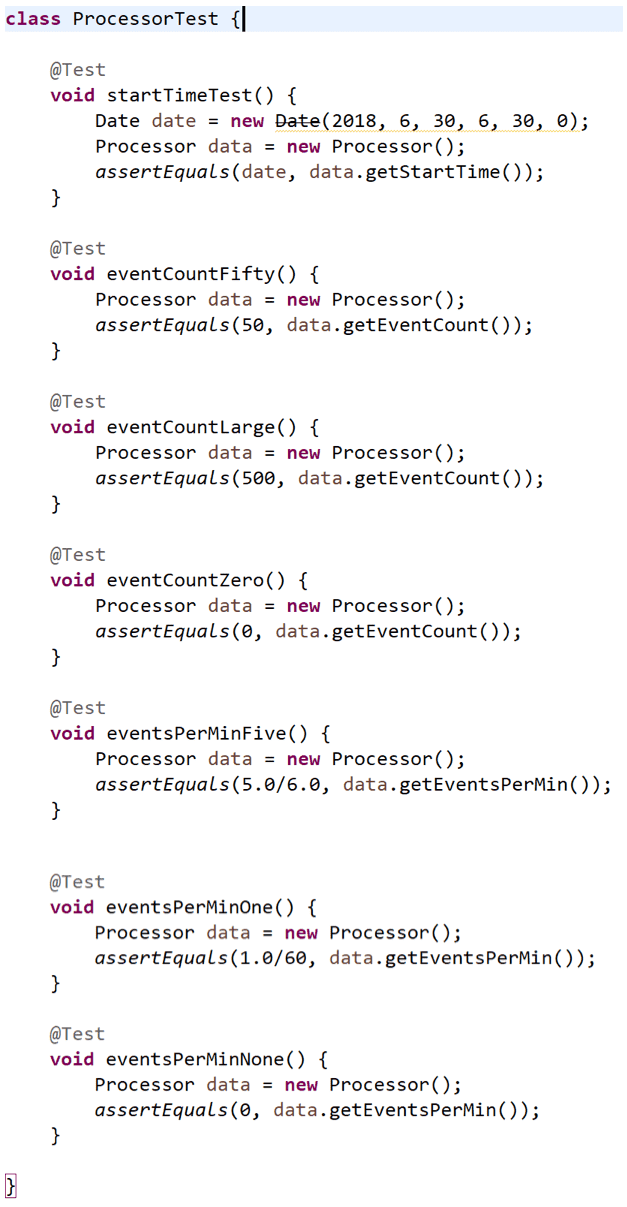
\includegraphics[width=0.63\textwidth]{codeimg1.png}  
\end{figure}

To compile the test code, a basic skeleton of the Processor class was created:

\begin{figure}[h]
	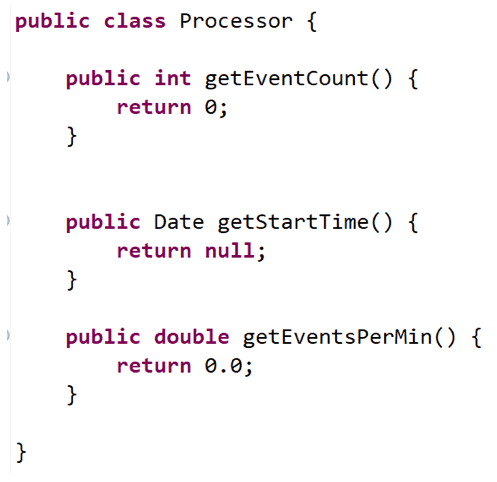
\includegraphics[width=0.63\textwidth]{codeimg2.png}
\end{figure}

When the previously created test class was now run, all but two of the tests failed. The only tests that passed already expected "0" as a result:

\begin{figure}[h]
	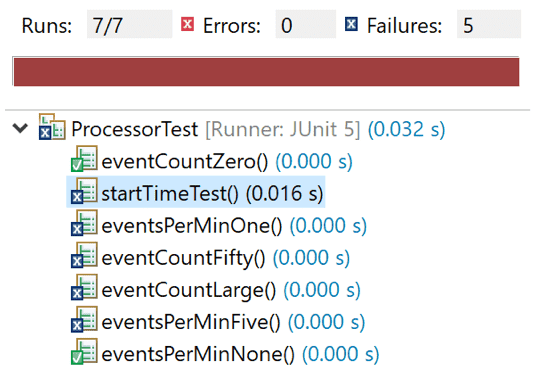
\includegraphics[width=0.83\textwidth]{codeimg3.png}
	\end{figure}
	
\newpage
\subsection*{3-2: Tests with Partial Implementation}

While working on the implementation, we realized that we needed more data and methods to flesh out the Processor class, resulting in an increased number of test cases. For example, to calculate events per minute, we needed to save the timestamps when data collection began and ended to know the length of time spent recording data. This functionality is performed by the new switchRecording method.
 
Although the full implementation of this requirement will use real muon event data from a connected muon detector, the test cases created fake data to simulate how real events would be saved by the Processor.

The following screenshots show some of the test cases after implementation:



\begin{figure}[h]
	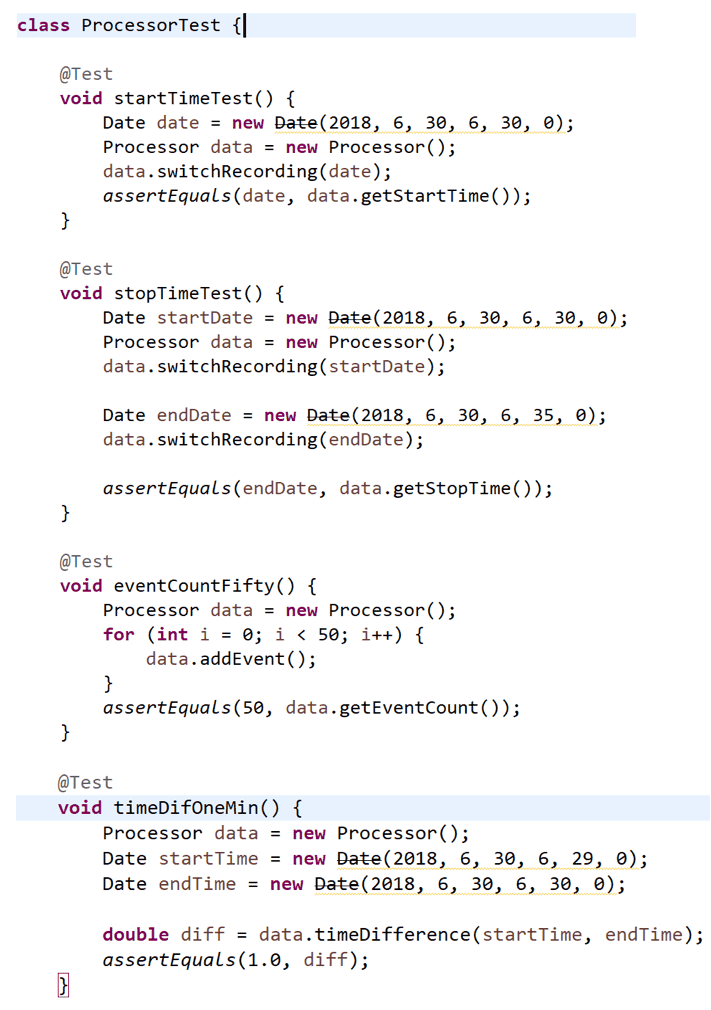
\includegraphics[width=0.79\textwidth]{codeimg4.png}
	\end{figure}

The new timeDifference method was created to calculate the difference between two timestamps in minutes. This is used in conjunction with the getEventsPerMin method:

\begin{figure}[h]
	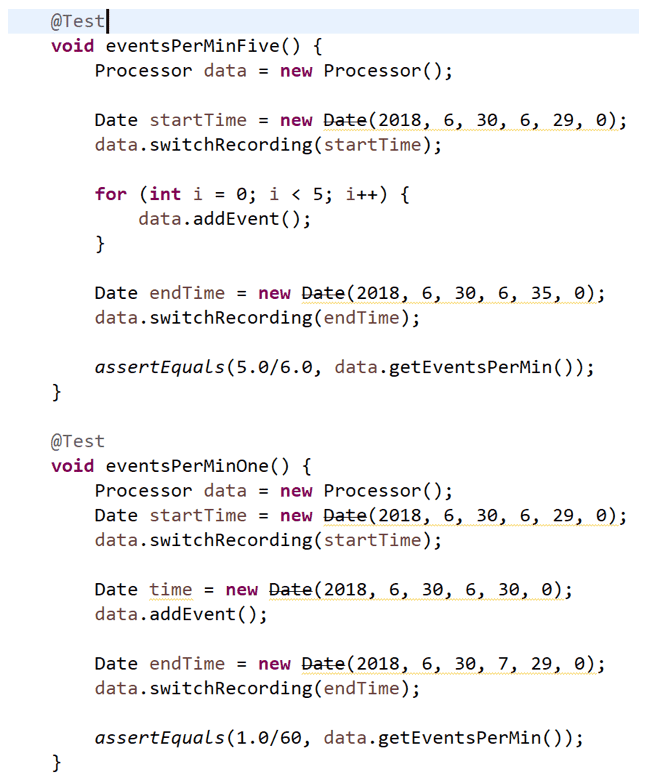
\includegraphics[width=1.0\textwidth]{codeimg5.png}
	\end{figure}
	
	
\newpage
The Processor class now has partially complete methods. However, it does not yet store instances of each muon event:

\begin{figure}[h]
	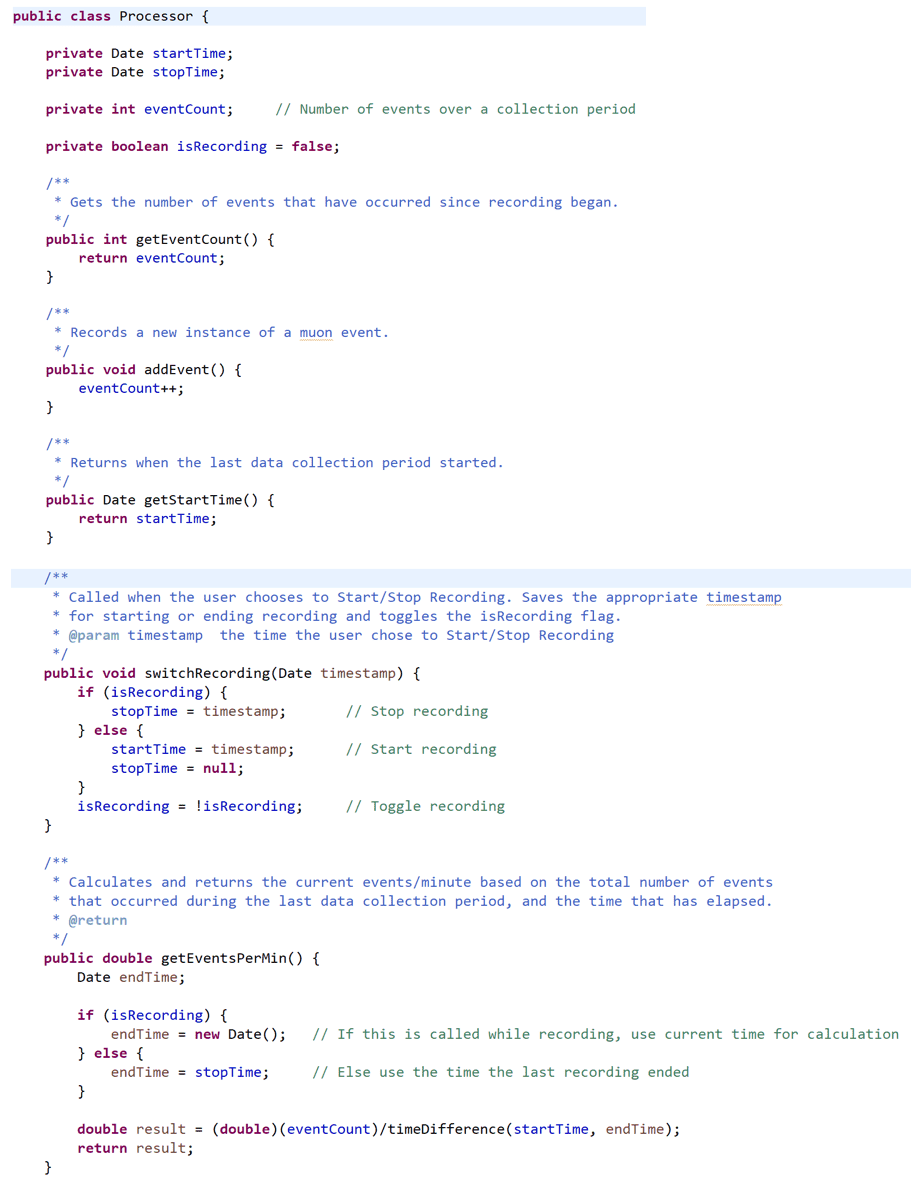
\includegraphics[width=1.1\textwidth]{codeimg6.png}
\end{figure}

\newpage

Now there is enough code to pass all the test cases:

\begin{figure}[h]
	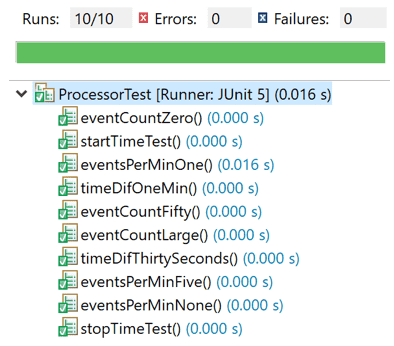
\includegraphics[width=0.7\textwidth]{codeimg7.png}
\end{figure}


\subsection*{3-3: Tests with Full Implementation}

Our demo video demonstrating the TDD approach with full implementation along with explanations can be viewed at the following (\href{https://www.youtube.com/watch?v=h2C-4-hQrhM&feature=youtu.be}{\underline{link}}).

\subsection*{3-4: Two Extra Functional Requirements}

Our demo video featuring all three functional requirements can be viewed at the following (\href{https://www.dropbox.com/s/vnuvuzx5zrtkvaa/Demo.mp4?dl=0}{\underline{link}}).



\newpage


\section*{Deliverable \#4}

\subsection*{4-1: Class Diagram}

\begin{figure}[h] \centering \hspace*{-3cm} \vspace{3cm}
	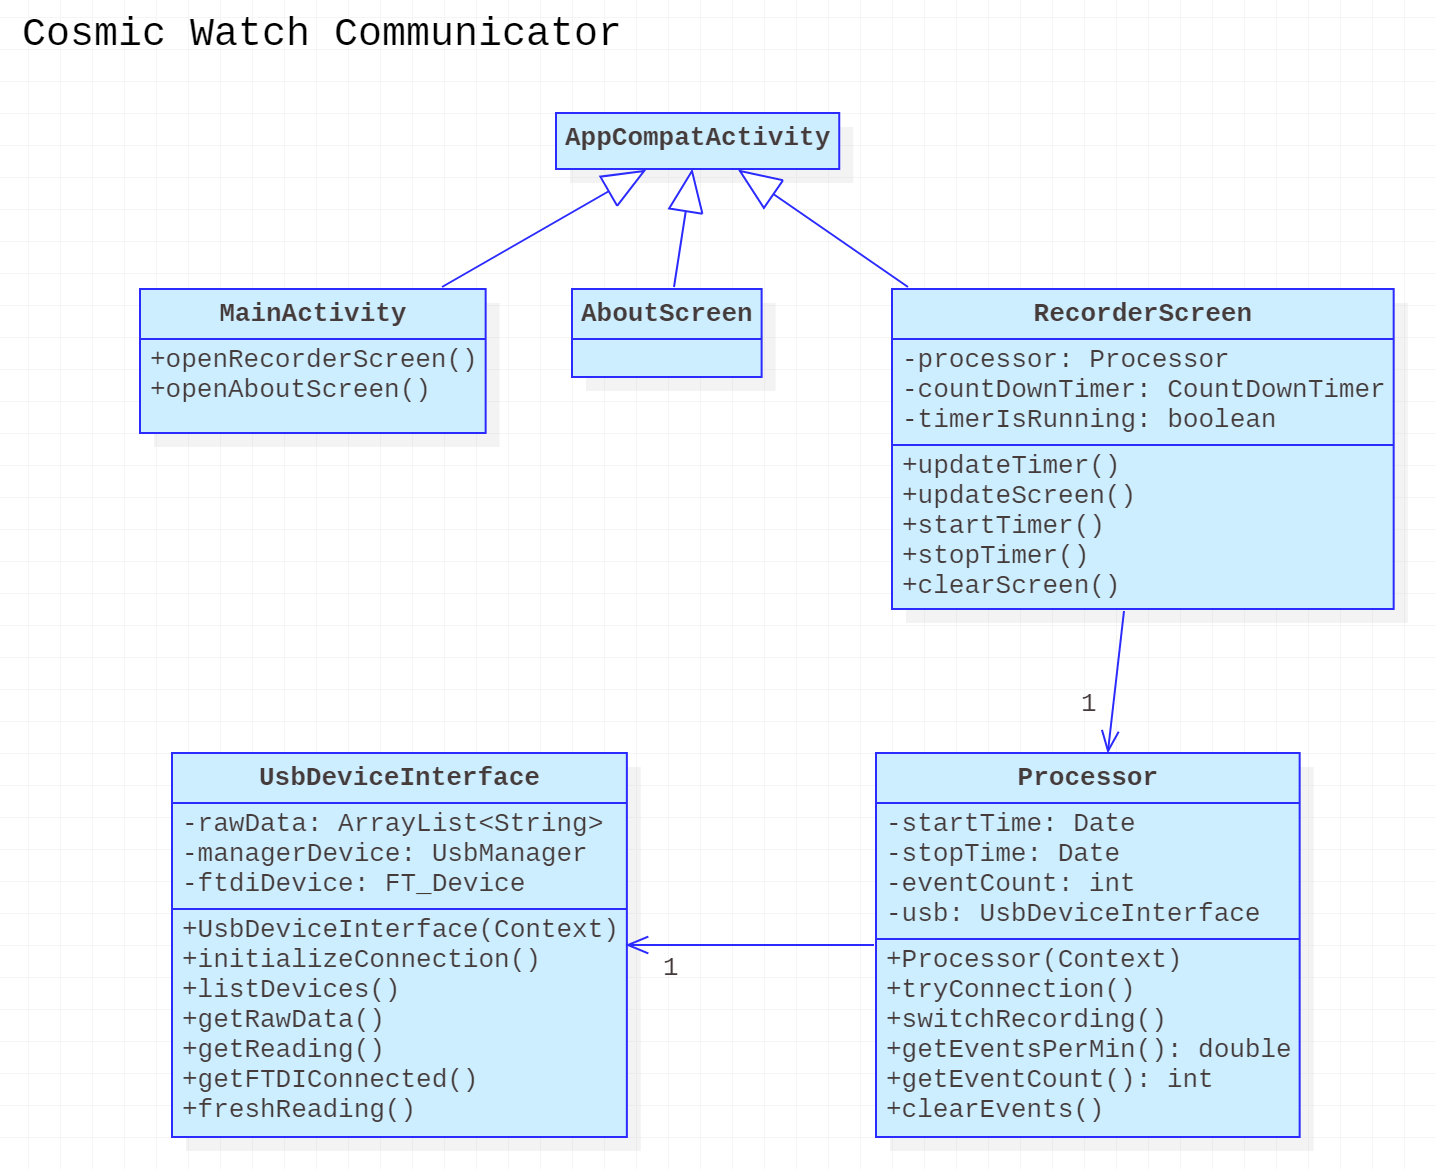
\includegraphics[width=1.5\textwidth]{classes.png}
\end{figure}
\newpage
\subsection*{4-2: Detailed Explanation}

At the top of our diagram, there are three classes extending the class AppCompatActivity. This indicates that these are the main Activities of our app, representing the screens the user can access; MainActivity, AboutScreen and RecorderScreen correspond to the Main Menu, About, and Recorder screens respectively.

The Main Menu screen allows the user to access the About and Recorder screens. Thus, MainActivity has the methods openRecorderScreen and openAboutScreen. The About screen simply displays information, so it does not have relevant attributes and operations to show.

RecorderScreen maintains a reference to a Processor object, which communicates between the UsbDeviceInterface and the RecorderScreen.

The RecorderScreen starts a timer when the user chooses to start recording. This is conveyed to the Processor, which will save the time recording starts and initialize the UsbDeviceInterface. The UsbDeviceInterface will open a wired connection to the muon detector and store raw data from it. When this data needs to be interpreted and displayed on the RecorderScreen, the Processor will make requests to the UsbDeviceInterface and update eventCount according to the amount of raw data saved.

When the recording session timer ends or when the user wishes to clear their saved data, the RecorderScreen sends another signal to Processor. The Processor will then reset its saved data and the raw data in UsbDeviceInterface as needed.


\newpage

\section*{Deliverable \#5}

\subsection*{5-1: Sequence Diagram 1 with Explanation}

\begin{figure}[h] \centering
	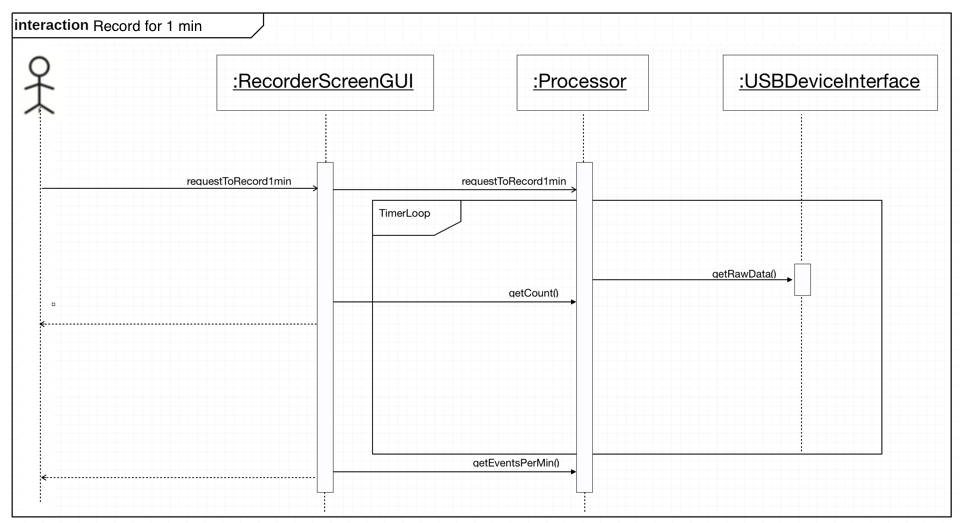
\includegraphics[width=1.08\textwidth]{sequence1.png}
\end{figure}

Our first sequence diagram demonstrates the sequence of tasks where a user initiates a recording for 1 minute. This is done by the user first being able to interact with a RecorderScreenGUI interface, specifically a button. The button communicates with the Processor class which creates a corresponding time stamp for the start of the recording session and enters into a TimerLoop for 60 seconds. During those 60 seconds, the Processor communicates with the USBDeviceInterface, which is a class used to communicate with an external piece of hardware known as a muon detector. 

As the muon detector picks up events, the Processor class calls getRawData() method from the USBDeviceInterface class increment events, which increases the private variable count in the Processor class. This happens every time a muon event occurs during those 60 seconds. The RecorderScreenGUI class then updates the count displayed by calling teh getCount() method from Processor. At the end of the TimerLoop, the RecorderScreenGUI calls the getEventsPerMin() method of the Processor class which calculates the total events that occurred divided by the total duration the recording took place by using the date stamp time difference. 

All of this information is then finally presented to the user in the RecorderScreenGUI. This entire sequence of tasks demonstrates a key concept in software engineering/computer science which is a layer of abstraction with all of the subsystems working behind the scenes while the user only interacts with a friendly UI. 

\newpage
\subsection*{5-2: Sequence Diagram 2 with Explanation}

\begin{figure}[h] \hspace{-2cm}
	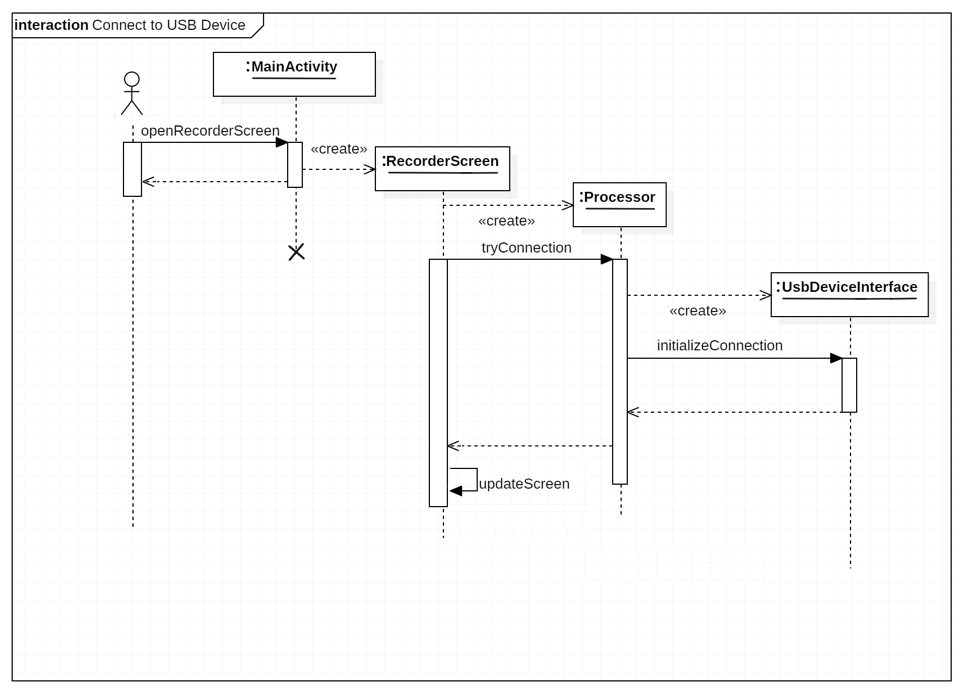
\includegraphics[width=1.3\textwidth]{sequence2.png}
\end{figure}


This sequence diagram shows the use case of the user successfully connecting to the muon detector through a USB port. When the user is on the Main Menu screen (MainActivity), they will choose to open the Recorder screen. This results in an instance of RecorderScreen being created, which also creates a Processor. MainActivity is no longer needed. 

Upon creation, RecorderScreen will ask the Processor to try to connect to the detector using the UsbDeviceInterface. The Processor will initialize the UsbDeviceInterface, and the UsbDeviceInterface will form the connection with the muon detector. After this connection is formed successfully, initializeConnection and tryConnection will return to the RecorderScreen. Finally, the RecorderScreen will display a message using updateScreen to show that the device is connected.


\newpage

\section*{Deliverable \#6}

\subsection*{6-1: Client Meeting}

We initially agreed to meet with Dr. Donev shortly after the completion of Assignment 1. However, we soon realized that we would not have much of our product complete by then, so we decided to hold the meeting later;

\begin{figure}[h] \centering
	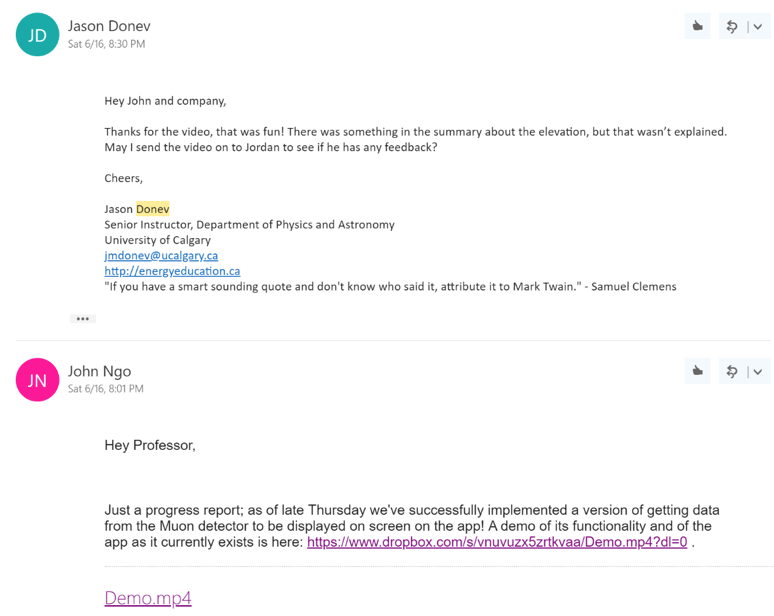
\includegraphics[width=1.1\textwidth]{email1.png}
\end{figure}

After we made more progress with implementation, we arranged a new time;

\begin{figure}[h] \centering
	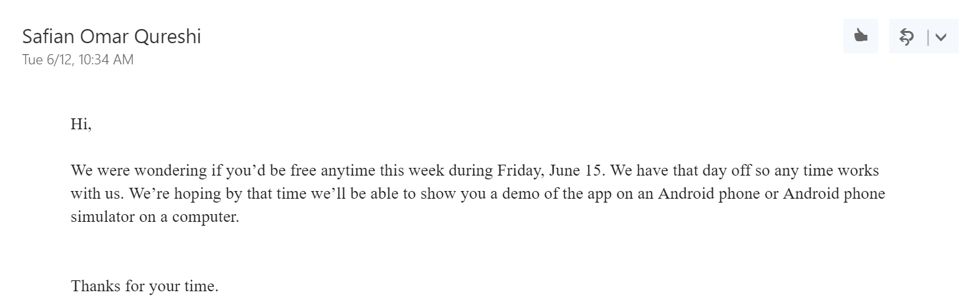
\includegraphics[width=1.2\textwidth]{email2.png}
\end{figure}

For our meeting, our app had two versions demonstrating different functional requirements that had yet to be integrated. We first showed that the app was able to connect to the muon detector via a mini-USB to mini-USB wired connection. We then showed the second version of the app, which could display fake data in a useful format to simulate what real data read from the muon detector would look like. We explained that we would combine these components to obtain one complete, functional product.

Dr. Donev was pleased by our progress and provided helpful feedback on our work. We allowed him to directly interact with the app’s simple interface on an Android tablet. He commented that a setting for the app that prevents the device from going to sleep while recording data would be useful; this was a feature we had not considered until testing the app on a real device. During this session, we also discovered some bugs with the interface. At the end of our meeting, we agreed to talk again on Monday to hopefully present a more polished product. 

Our greatest challenge in communicating with our customer was finding convenient times for all four of us to meet in-person. Although we spoke through email, some ideas could not be easily transferred through text alone. Due to our classes and Dr. Donev’s many obligations, we were not able to meet frequently. However, we made the most out of each meeting we had by focusing on obtaining as much feedback as possible from our client.







\end{document}